\newpage
\section{Pianificazione}\label{Pianificazione}
    La fase di \gloss{pianificazione} consiste nella suddivisione del lavoro tra i vari membri del gruppo. Essa deve fare in modo che ogni componente abbia la possibilità di ricoprire almeno una volta tutti i ruoli del progetto.\\
    Tenendo a mente le scadenze riportate nella sezione §1.4,
     AlphaSix ha ritenuto opportuno dividere il lavoro in quattro
     macro periodi:
     \begin{itemize}
		\item Analisi dei Requisiti
		\item Progettazione della Base Tecnologica
		\item Progettazione di dettaglio e codifica
		\item Validazione e Collaudo
     \end{itemize}
    
    In base al tipo di macro e al suo fine è stato deciso di scomporla in periodi più brevi per renderne più semplice il
    controllo e la pianificazione. AlphaSix per esemplificare l'intervallo di tempo tra una macro e l'altra usa vari
    diagrammi di Gantt\G dove sarà chiaro chi ha svolto qualsiasi attività. In ognuno di essi ci saranno due
    milestone di colore verde, la prima si riferisce alla consegna dei documenti e la successiva rappresenta la discussione di essi.

    \subsection{Analisi dei Requisiti}
        Questa macro ha inizio il 15-11-2018, procede con quattro periodi fino al 14-01-2019 con la consegna dei documenti e nel
        quinto e ultimo AlphaSix si prepara per la Revisione dei Requisiti del 21-01-2019. I ruoli attivi saranno: 
        \begin{itemize}
            \item Responsabile
            \item Amministratore
            \item Analista
            \item Verificatore.
        \end{itemize}
        Questa macro è stata divisa in cinque periodi:
		\begin{itemize}
			\item \textbf{I periodo}: dal 22-11-2018 al 02-12-2018
			\begin{itemize}
    	        \item \textbf{Discussione capitolati}: sono stati discussi pro e contro di ogni capitolato e dopo un periodo di
    	        studio e analisi il gruppo ha concluso con la scelta del capitolato C1 
    	        \item \textbf{Ricerca degli strumenti}: individuazione degli strumenti di supporto da utilizzare durante il progetto
    	        \item \textbf{Normazione}: definizione di regole per stilare i documenti
    	        \item \textbf{Distribuzione ruoli e pianificazione attività}
       	        \item \textbf{Studio di Fattibilità}
       	        \item \textbf{Pianificazione qualità}: individuazione metodi per garantire qualità del prodotto.
        	\end{itemize}
			\item \textbf{II periodo}: dal 03-12-2018 al 16-12-2018
			\begin{itemize}
    	        \item \textbf{Normazione}: definizione di regole per i processi organizzativi
    	        \item \textbf{Analisi dei requisiti}: ricerca requisiti del capitolato scelto
       	        \item \textbf{Ricerca degli strumenti}: individuazione strumenti per le varie attività di progetto
       	        \item \textbf{Pianificazione attività}: diagrammi di Gantt e pianificazione dell'intero progetto.
        	\end{itemize}
        	\item \textbf{III periodo}: dal 17-12-2018 al 29-12-2018
			\begin{itemize}
    	        \item \textbf{Normazione}: definizione di regole per i processi organizzativi
    	        \item \textbf{Definizione casi d'uso}
       	        \item \textbf{Ricerca degli strumenti}: strumenti per l'interfacciarsi a \gloss{Producers}, \gloss{Broker}.
        	\end{itemize}
        	\item \textbf{IV periodo}: dal 30-12-2018 al 13-01-2019
        	\begin{itemize}
    	        \item \textbf{Analisi dei rischi}
       	        \item \textbf{Ricerca degli strumenti}: strumenti per l'interfacciarsi con il Gestore del personale, \gloss{Consumers}
       	        \item \textbf{Pianificazione attività}: aggiornamenti della pianificazione
       	        \item \textbf{Stesura lettera di presentazione}.
        	\end{itemize}
        	\item \textbf{V periodo}: dal 15-01-2019 al 20-01-2019
        	\begin{itemize}
    	        \item \textbf{Preparazione per la discussione}: implementazione slide della presentazione e studio. personale
        	\end{itemize}
		\end{itemize}
		
        \begin{landscape}
			\subsubsection{Diagramma di Gantt}        
			\begin{figure}[H]
					\centering
					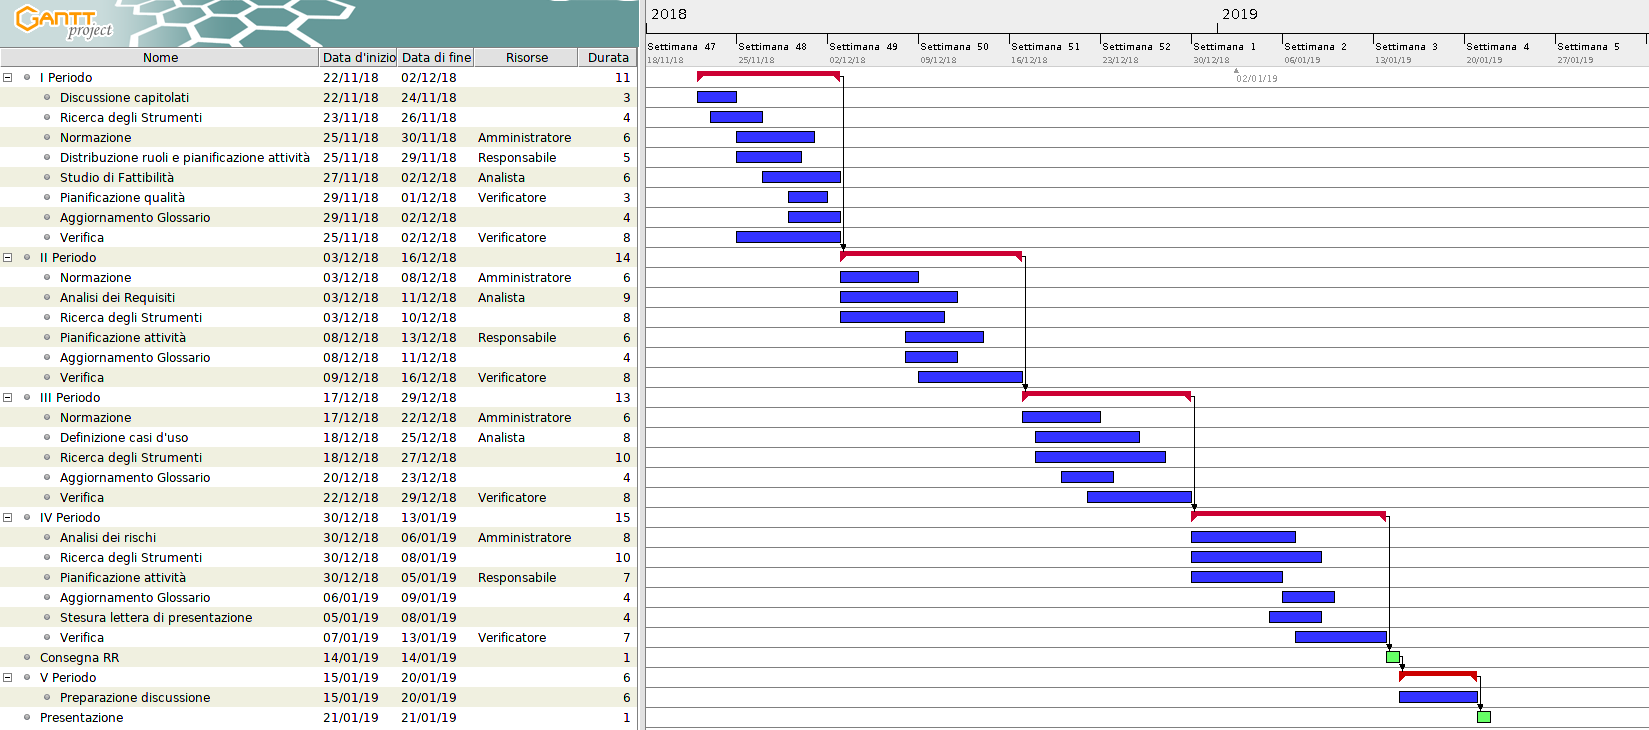
\includegraphics[scale=0.425]{img/Analisi_dei_Requisiti.png}\\
					\caption{Diagramma di Gantt della macro Analisi dei Requisiti}
			\end{figure}
		\end{landscape}
		\newpage
        \subsection{Progettazione della Base Tecnologica}
        	Questa macro ha inizio il 22-01-2019, procede con due periodi fino al 08-03-2019 con la consegna dei documenti e nel
        terzo e ultimo AlphaSix si prepara per la Revisione di Progetto del 15-03-2019. I ruoli attivi saranno: 
        \begin{itemize}
            \item Responsabile
            \item Amministratore
            \item Analista
            \item Progettista
            \item Programmatore
            \item Verificatore.
        \end{itemize}
        Questa macro è stata divisa in tre periodi:
		\begin{itemize}
			\item \textbf{I periodo}: dal 22-01-2019 al 03-02-2019
			\begin{itemize}
    	        \item \textbf{Normazione}
    	        \item \textbf{Analisi dei Requisiti}
    	        \item \textbf{Pianificazione attività}: aggiornamenti pianificazione
    	        \item \textbf{Pianificazione della qualità}
    	        \item \textbf{Progettazione}: implementazione schemi UML.
        	\end{itemize}
			\item \textbf{II periodo}: dal 04-02-2019 al 07-03-2019
			\begin{itemize}
				\item \textbf{Ricerca degli strumenti}: \gloss{Apache Kafka}, \gloss{Docker}, gloss{API Rest} 
    	        \item \textbf{Normazione}: aggiunta nuovi strumenti utilizzati
    	        \item \textbf{Proof of Concept}: implementazione che rappresenti la Baseline
    	        \item \textbf{Technology Baseline}: tecnologie, framework e librerie per lo sviluppo del prodotto
    	        \item \textbf{Pianificazione delle attività}: aggiornamenti della pianificazione
    	        \item \textbf{Codifica}: realizzazione del Proof of Concept
    	        \item \textbf{Stesura lettera di presentazione}.
        	\end{itemize}
        	\item \textbf{III periodo}: dal 09-03-2019 al 14-03-2019
			\begin{itemize}
				\item \textbf{Preparazione per la discussione}: implementazione slide della presentazione e studio personale.
        	\end{itemize}
		\end{itemize}
        
        \begin{landscape}
			\subsubsection{Diagramma di Gantt}        
			\begin{figure}[H]
					\centering
					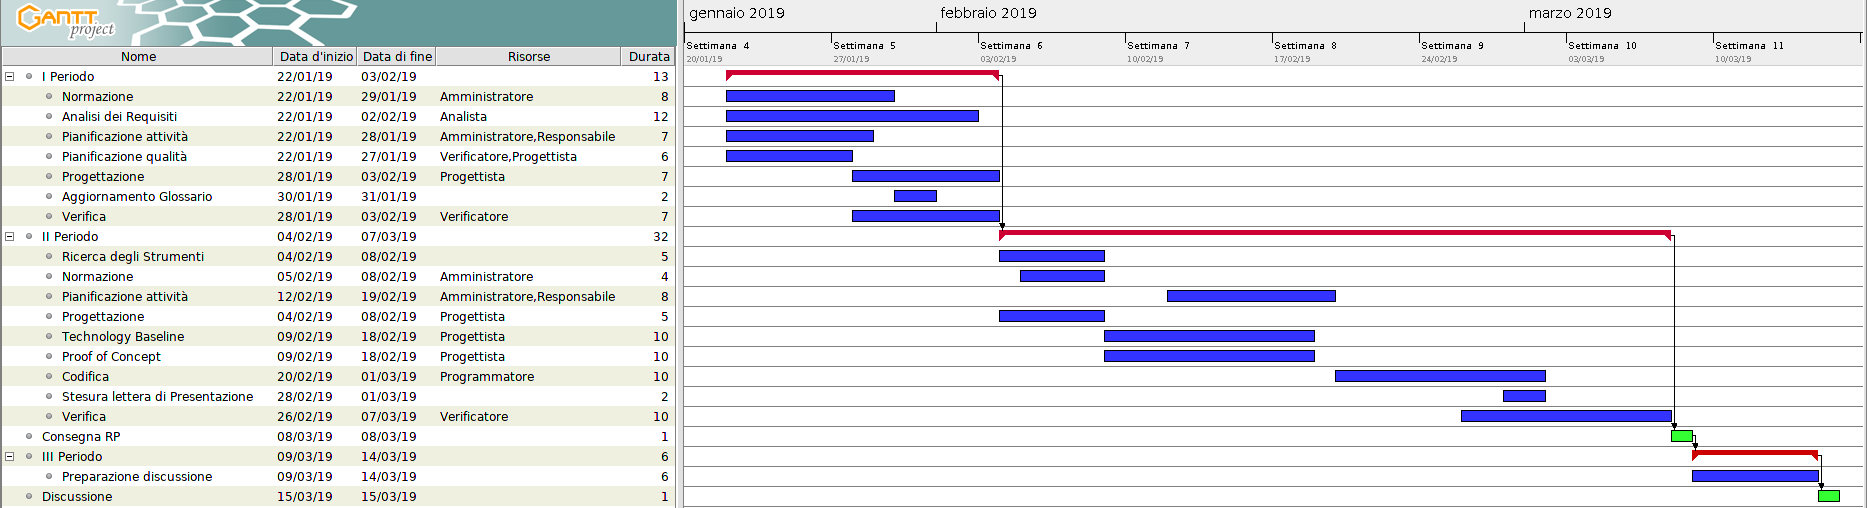
\includegraphics[scale=0.49]{img/Progettazione_della_base_tecnologica.png}\\
					\caption{Diagramma di Gantt della macro Progettazione della Base Tecnologica}
			\end{figure}
		\end{landscape}
		\newpage

        \subsection{Progettazione di dettaglio e codifica}
        Questa macro ha inizio il 16-03-2019, procede con tre periodi fino al 26-03-2019 con la consegna dei documenti e nel
        quarto e ultimo AlphaSix si prepara per la Revisione di Qualifica del 19-04-2019. I ruoli attivi saranno: 
        \begin{itemize}
            \item Responsabile
            \item Amministratore
            \item Progettista
            \item Programmatore
            \item Verificatore.
        \end{itemize}
        Questa macro è stata divisa in tre periodi:
		\begin{itemize}
			\item \textbf{I periodo}: dal 16-03-2019 al 26-03-2019
			\begin{itemize}
    	        \item \textbf{Ricerca degli Strumenti}
    	        \item \textbf{Pianificazione attività}: aggiornamenti pianificazione
    	        \item \textbf{Normazione}
    	        \item \textbf{Progettazione}: miglioramento Technology Baseline e Proof of Concept
    	        \item \textbf{Codifica}: prima implementazione.
        	\end{itemize}
			\item \textbf{II periodo}: dal 27-03-2019 al 03-04-2019
			\begin{itemize}
				\item \textbf{Progettazione e Product Baseline}: implementazione Product Baseline tramite diagrammi delle classi e di sequenza
				coerentemente con quanto dichiarato nella Technology Baseline
    	        \item \textbf{Normazione}
    	        \item \textbf{Codifica}: implementazione seguendo specifiche progettuali e implementazione test
    	        \item \textbf{Scrittura manuale}: prima stesura.
        	\end{itemize}
        	\item \textbf{III periodo}: dal 04-04-2019 al 11-04-2019
			\begin{itemize}
				\item \textbf{Pianificazione attività}: aggiornamenti pianificazione
    	        \item \textbf{Progettazione}: finalizzazione scelta dei \gloss{design pattern}
    	        \item \textbf{Codifica}: primo rilascio
    	        \item \textbf{Scritura manuale}: aggiornamenti al manuale
    	        \item \textbf{Stesura lettera di presentazione}.
        	\end{itemize}
        	\item \textbf{IV periodo}: dal 13-04-2019 al 18-04-2019
			\begin{itemize}
				\item \textbf{Preparazione per la discussione}: implementazione slide della presentazione e studio personale.
        	\end{itemize}
        \end{itemize}

        \begin{landscape}
			\subsubsection{Diagramma di Gantt}        
			\begin{figure}[H]
					\centering
					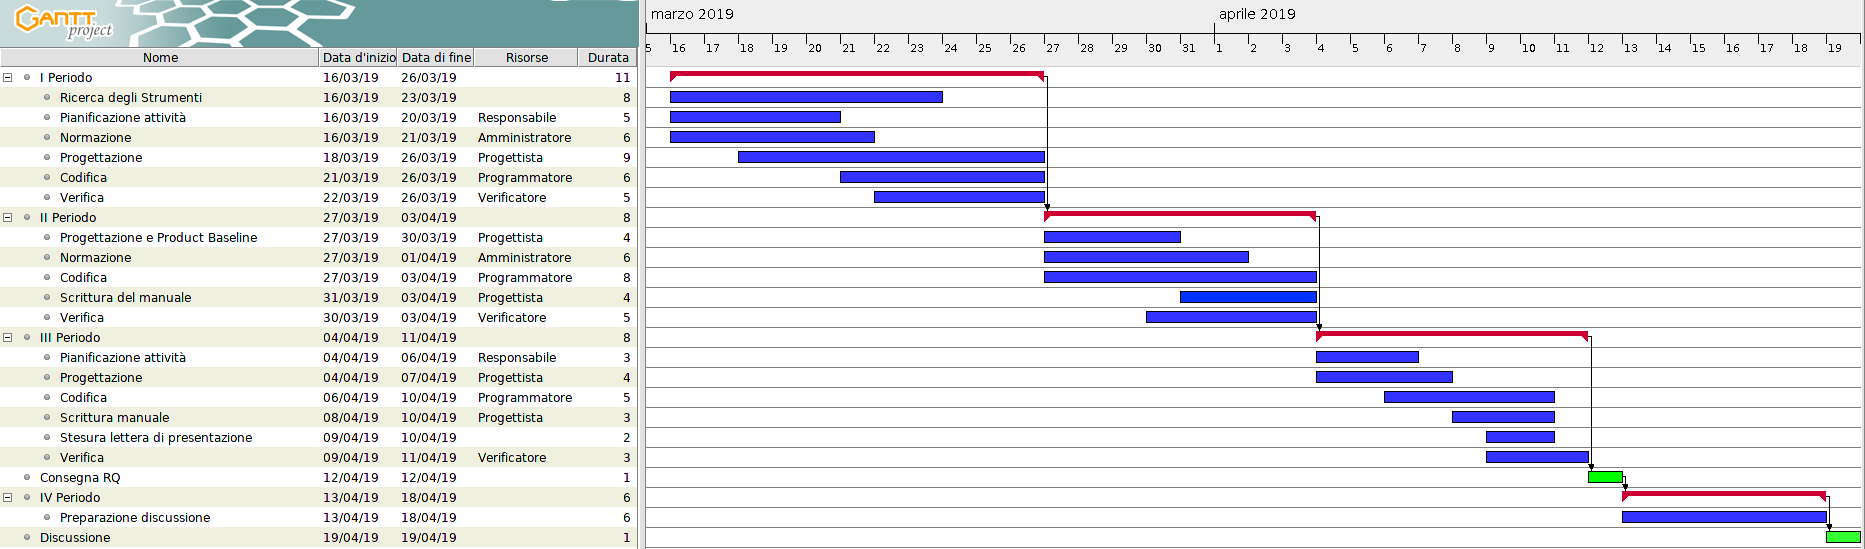
\includegraphics[scale=0.44]{img/Progettazione_di_dettaglio_e_codifica.png}\\
					\caption{Diagramma di Gantt della macro Progettazione di dettaglio e codifica}
			\end{figure}
		\end{landscape}
		\newpage

        \subsection{Validazione e Collaudo}
        Questa macro ha inizio il 20-04-2019, procede con due periodi fino al 16-05-2019 con la consegna dei documenti e AlphaSix si
        prepara per la Revisione di Accettazione del 17-05-2019. I ruoli attivi saranno: 
        \begin{itemize}
            \item Amministratore
            \item Analista
            \item Progettista
            \item Programmatore
            \item Verificatore.
        \end{itemize}
        Questa macro è stata divisa in due periodi:
		\begin{itemize}
			\item \textbf{I periodo}: dal 20-04-2019 al 30-04-2019
			\begin{itemize}
    	        \item \textbf{Normazione}
    	        \item \textbf{Analisi dei requisiti}
    	        \item \textbf{Pianificazione attività}: aggiornamenti pianificazione
    	        \item \textbf{Pianificazione della qualità}
    	        \item \textbf{Progettazione Technology Baseline e Product Baseline}: completamento delle specifiche
        	\end{itemize}
			\item \textbf{II periodo}: dal 01-05-2019 al 15-05-2019
			\begin{itemize}
    	        \item \textbf{Codifica}: completamento ultima versione
    	        \item \textbf{Scrittura manuale}: completamento manuale
    	        \item \textbf{Test e collaudo}: esecuzione di test di qualifica e ultimi miglioramenti del prodotto per
    	        garantire che il prodotto soddisfi tutti i vincoli qualitativi.
    	        \item \textbf{Preparazione discussione}
        	\end{itemize}
		\end{itemize}
        
        \begin{landscape}
			\subsubsection{Diagramma di Gantt}        
			\begin{figure}[H]
					\centering
					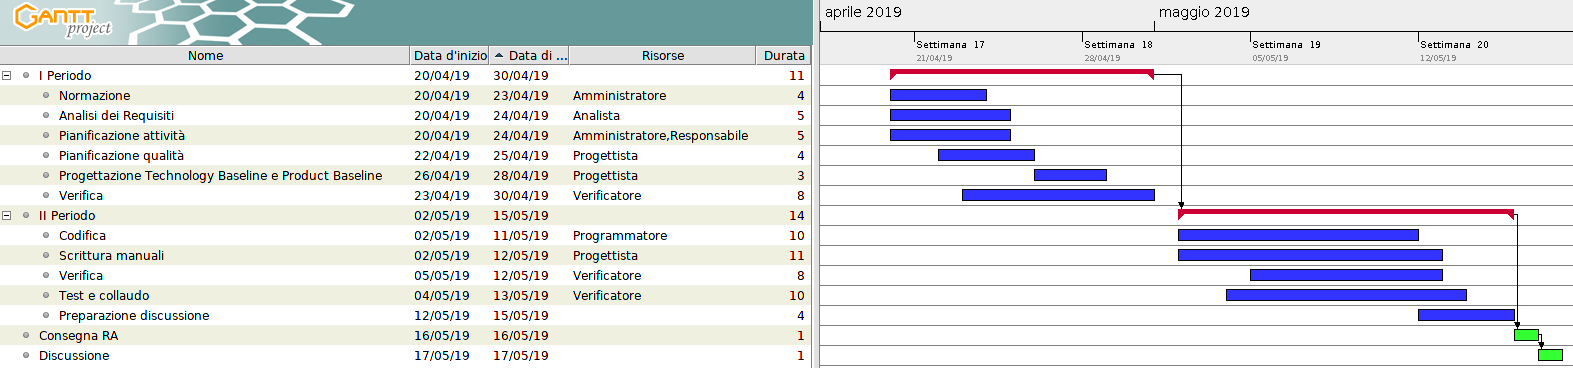
\includegraphics[scale=0.44]{img/Validazione_e_collaudo.png}\\
					\caption{Diagramma di Gantt della macro Validazione e Collaudo}
			\end{figure}
		\end{landscape}
		\newpage
